%\vspace{-0.05in}
\subsection{Experimental Results}
\label{results}
%\vspace{-0.05in}

Figure~\ref{fig:annotated} shows the results of using our feedback-based
optimization compiler workflow and annotating our workloads using our new page
placement interfaces. We found that on our capacity-limited machine, 
annotation-based placement outperforms the Linux INTERLEAVE policy 
performance by 19\% and naive BW-AWARE 30C-70B placement by 14\%
on average.  Combining program annotated placement hints and our runtime placement engine 
achieves 90\% of oracular page placement on average.  In all cases
our program-annotated page placement algorithm outperforms BW-AWARE placement, making
it a viable candidate for optimization beyond BW-AWARE placement if programmers choose to
optimize for heterogeneous memory system properties.

\begin{figure}[t]
    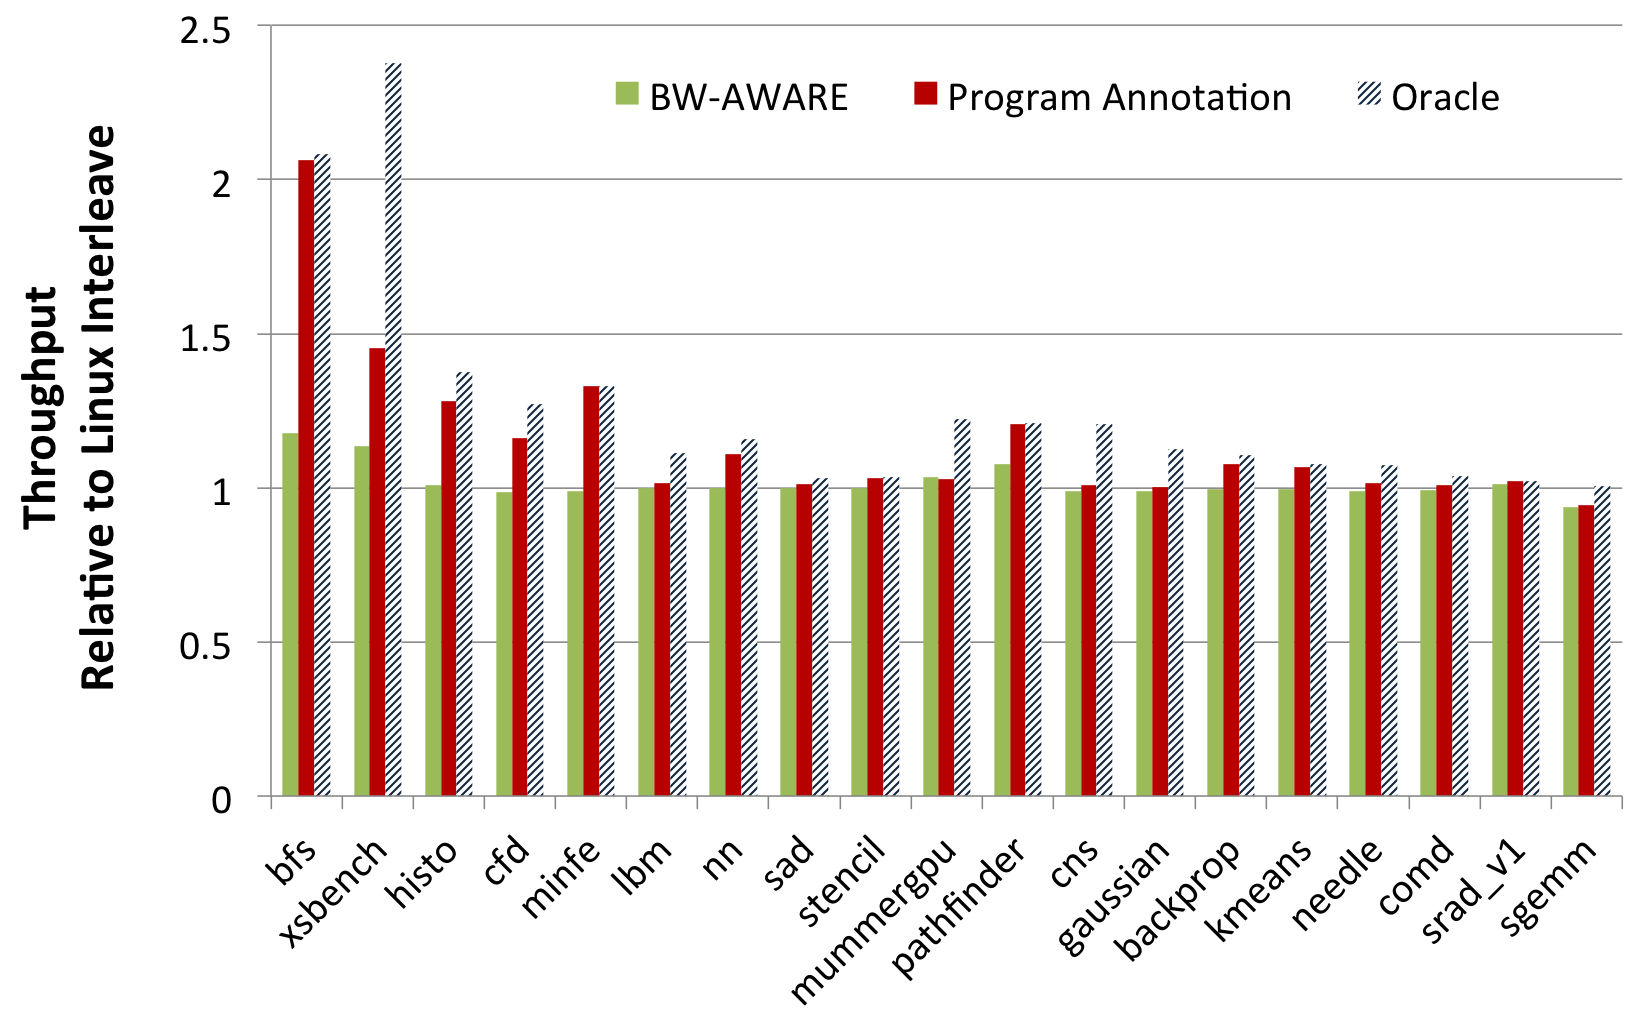
\includegraphics[width=\columnwidth]{asplos2015/figures/appannotated-10per.png}
    \caption{Profile-driven annotated page placement performance relative to INTERLEAVE, BW-AWARE and oracular policies
    under at 10\% capacity constraint.}
    \label{fig:annotated}
\end{figure}

One of the drawbacks to profile-driven optimization is that data dependent
runtime characteristics may cause different behaviors than were seen during
the profiling phase. While GPU applications in production will be run without code
modification, the data set and parameters of the workload typically vary in both
size and value from run-to-run.
Figure~\ref{fig:sensitivitytotraining} shows the sensitivity of our workload performance to
data input set changes, where placement was trained on the first data-set but
compared to the oracle placement for each individual dataset.
We show results for the four example applications which saw the highest improvement
of oracle placement over BW-AWARE.\@ For {\tt bfs}, we varied the number 
of nodes and average degree of the graph.
For {\tt xsbench}, we changed three parameters: number of nuclides, number of
lookups, and number of gridpoints in the data set. For {\tt minife}, we varied
the dimensions of the finite element problem by changing the input matrix.
Finally, for {\tt mummergpu}, we changed the number of queries and length of
queries across different input data sets.

Using the profiled information from only the training set, we observe that annotated
placement performs 29\% better than the baseline Linux INTERLEAVE policy,
performs 16\% better than our 
own BW-AWARE 30C-70B placement, and achieves 80\% of the oracle placement performance.  This 
result indicates that for GPU compute applications, feedback-driven optimization for page placement
is not overly sensitive to application dataset or parameter variation, although pessimistic
cases can surely be constructed.


%\vspace{-0.05in}
\subsection{Discussion}
\vspace{-0.05in}
The places where annotation-based placement falls short primarily come from
three sources.  First, our application profiling relies on spatial locality of virtual addresses 
to determine page hotness.  We have shown that this spatial locality holds true
for many GPU applications, but this is not guaranteed to always be the case. Allocations within 
libraries or larger memory ranges the programmer chooses
to logically sub-allocate within the program will not exhibit this property. 
The second shortcoming of our annotation-based approach is for applications 
which show high variance within a single data structure.  {\color{black}For example, when using a hashtable 
where the application primarily accesses a small, dynamically determined portion of the total key-space,
our static hotness profiling will fail to distinguish the hot and cold regions of this structure}.  Finally,
although our runtime system abstracts the programming challenges of writing
performance portable code for heterogeneous machines, it is still complex and puts
a large onus on the programmer.  Future work will be to learn from our current
implementation and identify mechanisms to reduce the complexity we expose to the programmer
while still making near-ideal page placement decisions.

\begin{figure}[t]
    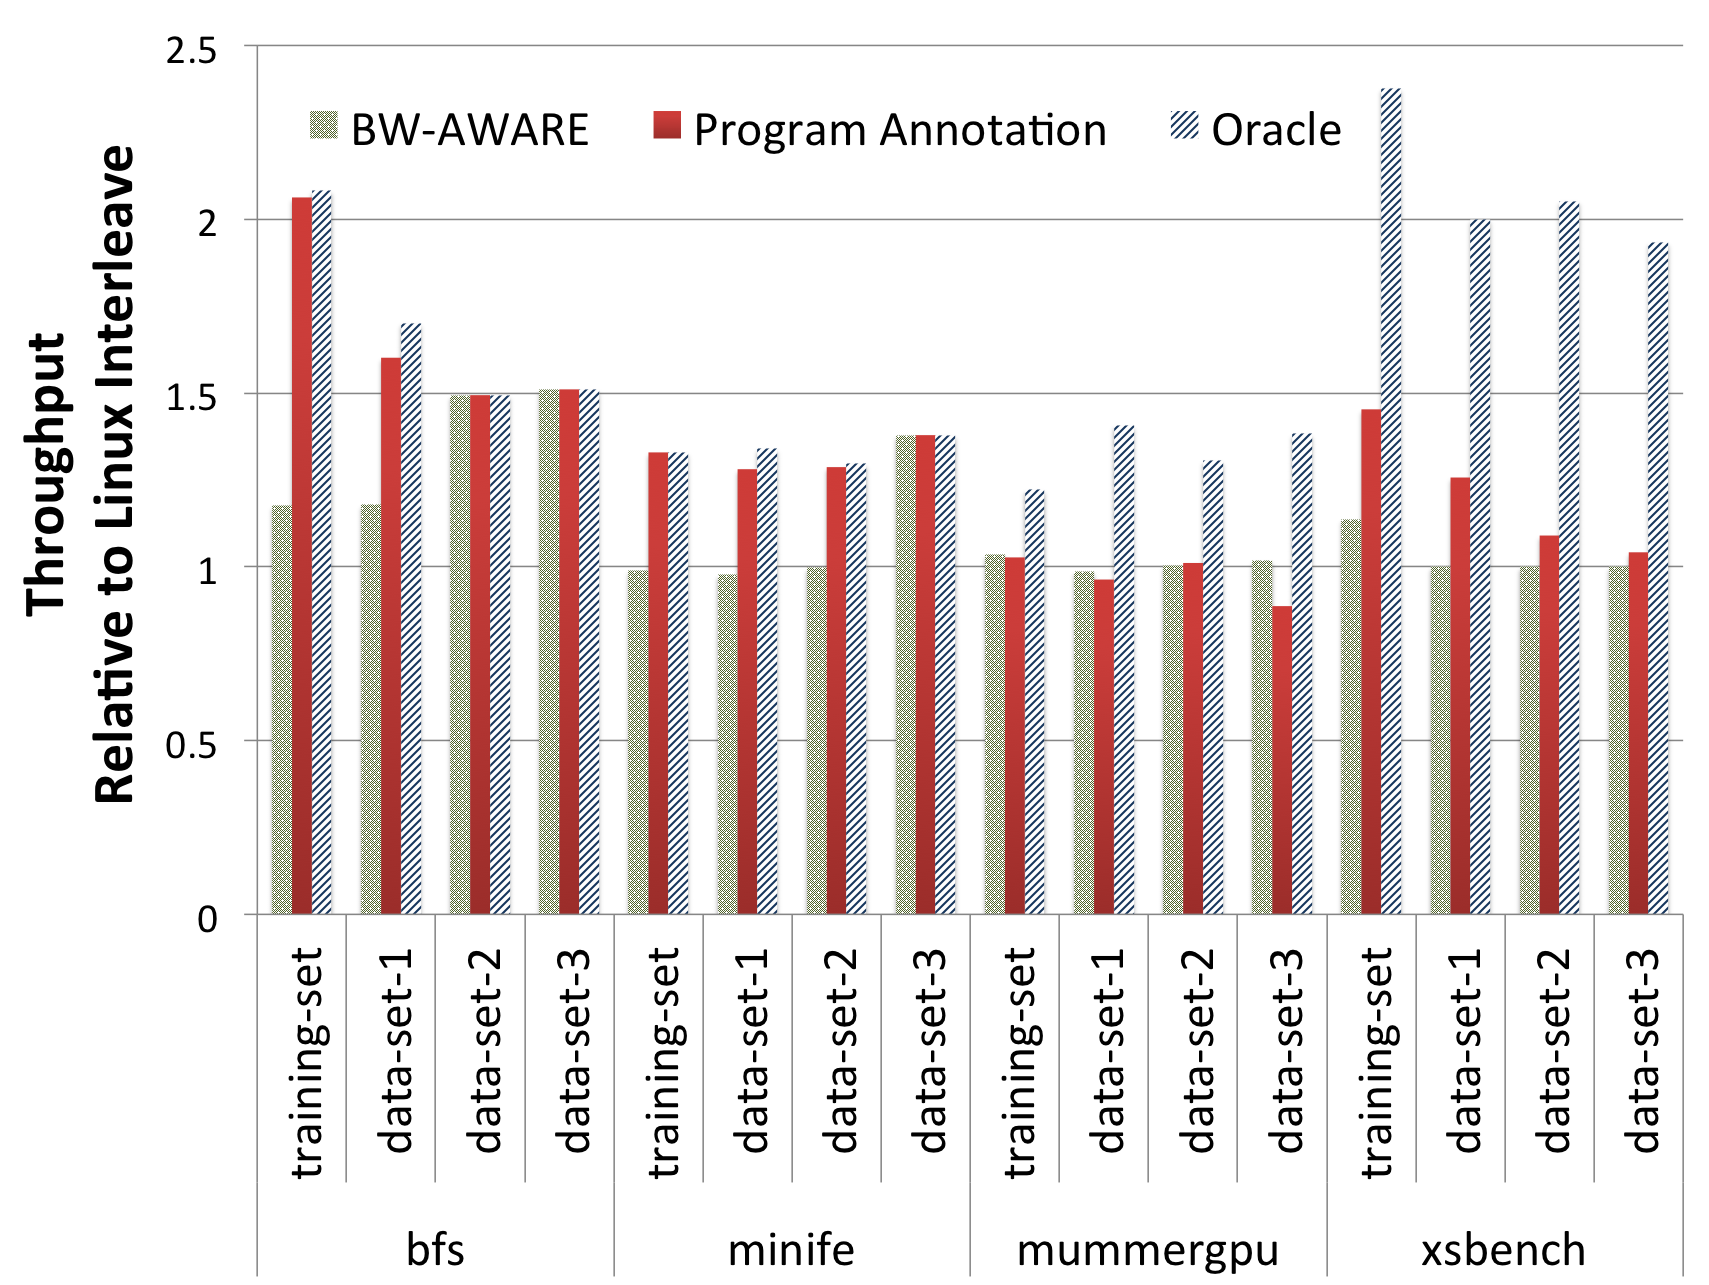
\includegraphics[width=\columnwidth]{asplos2015/figures/sensitivitytotraining.png}
    \caption{Annotated page placement effectiveness versus data sets variation after training phase under at 10\% capacity constraint.}
    \label{fig:sensitivitytotraining}
\end{figure}

In this work we have focused on page placement for applications assuming a static
placement of pages throughout the application runtime. We recognize that temporal phasing in
applications may allow further performance improvement but have chosen to focus
on initial page placement rather than page migration for two reasons.  First,
software-based page migration is a very expensive operation.  Our measurements on the Linux 3.16-rc4 
kernel indicate that it is not possible to migrate pages between NUMA memory zones at a rate faster
than several GB/s and with several microseconds of latency between invalidation and first
re-use.  While GPUs can cover several hundred nanoseconds of memory latency, microsecond
latencies encountered during migration will induce high overhead stalls within the compute pipeline.
Second, online page migration occurs only after some initial placement decisions have been
made.  Focusing on online page migration before finding an optimized initial placement policy
is putting the cart before of the horse.  With improved default page placement
for GPU workloads, the need for dynamic page migration is reduced.  Further work is needed 
to determine if there is significant value to justify the expense of online profiling 
and page-migration for GPUs beyond improved initial page allocation.
